\documentclass{beamer}
\beamertemplatenavigationsymbolsempty
\usepackage{graphicx, tikz}


\begin{document}


\begin{frame}{Chromatic Polynomial}
  Rather than just knowing whether we \emph{can} colour a graph $G$ with $k$ colours, we can count the different colourings that are possible.

  \begin{definition}Let $G$ be a simple (why?) graph, and let $k\geq 1$ be an integer.  The \emph{chromatic polynomial} $P_G(k)$ is the number of different ways to colour the vertices of $G$ with $k$ colours, so that adjacent vertices have different colours.
  \end{definition}

  \begin{block}{Remarks:}
    \begin{itemize}
    \item It is \emph{not} obvious from the definition that $P_G(k)$ is a polynomial
    \item $P_G(k)=0\iff 0\leq k <\chi(G)$
    \end{itemize}
    \end{block}
\end{frame}  

\begin{frame}{In easy examples, can colour vertex by vertex:}
\begin{block}{Colour vertex $v_1$, then vertices adjacent to $v_1$, then..}
  

  \begin{itemize}
  \item $P_{E_n}(k)=k^n$
  \item $P_{K_n}(k)=k(k-1)(k-2)\cdots (k-n+1)$
  \item If $T$ is a tree with $n$ vertices, then $P_T(k)=k(k-1)^n$
  \end{itemize}
  \end{block}
  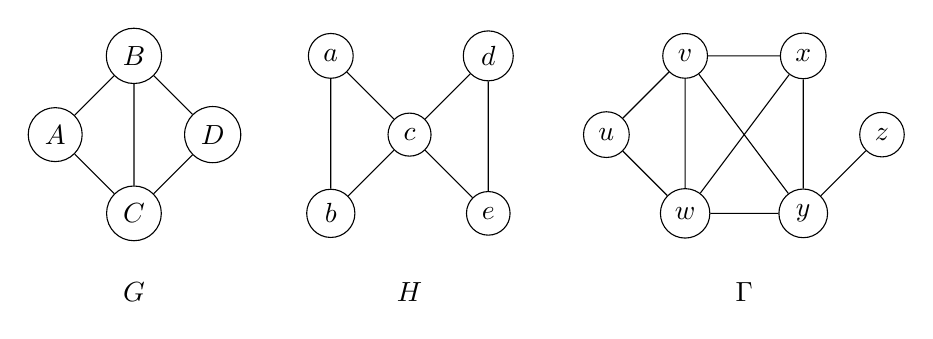
\begin{tikzpicture}
    \node at (1,-2) {$G$};
    \node at (4.5, -2) {$H$};
    \node at (8.75, -2) {$\Gamma$};
    
    \begin{scope}[every node/.style={circle, draw}]
      \node (A) at (0,0) {$A$};
      \node (B) at (1,1) {$B$};
      \node (C) at (1,-1) {$C$};
      \node (D) at (2,0) {$D$};
  \draw (B)--(A)--(C)--(D)--(B)--(C);    

    \begin{scope}[xshift=3.5cm]
   \node (a) at (0,1) {$a$};
      \node (b) at (0,-1) {$b$};
      \node (c) at (1,0) {$c$};
      \node (d) at (2,1) {$d$};
      \node (e) at (2,-1) {$e$};

      \draw (c)--(a)--(b)--(c)--(d)--(e)--(c);
            \end{scope}


    \begin{scope}[xshift=7cm]
      \node (u) at (0,0) {$u$};
      \node (v) at (1,1) {$v$};
      \node (w) at (1,-1) {$w$};
      \node (x) at (2.5,1) {$x$};
      \node (y) at (2.5,-1) {$y$};
      \node (z) at (3.5,0) {$z$};
      
    \draw (z)--(y)--(w)--(u)--(v)--(w)--(x)--(y)--(v)--(x);  


      \end{scope}
\end{scope}
    
    \end{tikzpicture}
  \begin{block}{What patterns do you notice?}
    \end{block}
\end{frame}

\begin{frame}{A harder example: $C_4$}
\begin{columns}
  \begin{column}{.2\textwidth}
        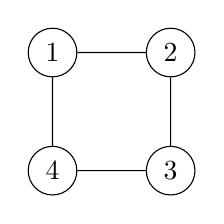
\begin{tikzpicture}
          \begin{scope}[every node/.style={circle, draw}, scale=1.5]
          \node (1) at (0,1) {$1$};
          \node (2) at (1,1) {$2$};
          \node (3) at (1,0) {$3$};
          \node (4) at (0,0) {$4$};
          \draw (1)--(2)--(3)--(4)--(1);
          \end{scope}
          \end{tikzpicture}
        \end{column} 

  \begin{column}{.7\textwidth}
        \begin{itemize}
        \item $k$ ways to colour vertex 1
        \item $k-1$ ways to colour vertex 2
        \item $k-1$ ways to colour vertex 3
        \item Don't know if $v_1$ and $v_3$ have same colour 
      \end{itemize}
\end{column}
    \end{columns}

  \begin{block}{Case 1: $v_1$ and $v_3$ have the same colour}
    \begin{itemize}
    \item $k$ choices for this colour
    \item Then $k-1$ choices for each of $v_2$ and $v_4$
    \end{itemize}
    \end{block}
  \begin{block}{Case 2: $v_1$ and $v_3$ have the same colour}
    \begin{itemize}
    \item $k$ choices for $v_1$, then $k-1$ choices for $v_3$
    \item $k-2$ choices for each of $v_2$ and $v_4$
    \end{itemize}
    \end{block}
Combining the cases, we see:
  $$P_{C_4}=k(k-1)^2+k(k-1)(k-2)^2=k(k-1)(k^2-3k+3)$$  
         \end{frame}

\begin{frame}{Foreshadowing: the two cases are chromatic polynomials}
  The type of reasoning we used to find the chromatic polynomial of $C_4$ will work to find the chromatic polynomial of any graph; however, many cases might need to be considered, and the argument will get quite complicated.

  \begin{block}{It will help to repackage the reasoning}
    \end{block}

  \begin{block}{Case 1: $v_1$ and $v_2$ are the same colour}
If they're the same colour, then we can make them same vertex...
        \end{block}
  
  \begin{block}{Case 2: $V_2$ and $v_3$ are different colours}
        If there's an edge between two vertices, then they need to be different colours.
  \end{block}

\end{frame}

\begin{frame}{Generalizing the observation we just made}
  
  \begin{block}{A lemma, with some definitions baked in}
    Suppose that $G$ is a graph, and $x$ and $y$ are two vertices that aren't adjacent. Define:
    \begin{itemize}
    \item  $G_{+xy}$ to be the graph with the edge $xy$ added
    \item $G_{x=y}$ to be the graph with $x$ and $y$ identified
    \end{itemize}
    Then:
    $$P_G(k)=P_{G_{+xy}}(k)+P_{G_{x=y}}(k)$$
  \end{block}

  \begin{proof} Consider a colouring of $G$; in some of them $x$ and $y$ will have different colourings, and in others $x$ and $y$ will have the same colour.  The colourings in the first case are exactly the colourings of $G_{+xy}$, the colourings in the second are the colourings of $G_{x=y}$.
   \end{proof}
    
    \end{frame}
\begin{frame}{The chromatic polynomial of $C_5$}
  \begin{columns}
    \begin{column}{.3\textwidth}
  \begin{tikzpicture}
    \begin{scope}[every node/.style={circle, draw}]
      \foreach \x in {1,2,...,5}{
        \node (\x) at (162-72*\x:1.5) {$\x$}}
      \draw (1)--(2)--(3)--(4)--(5)--(1);

    \end{scope}
    \end{tikzpicture}
    \end{column}

    \begin{column}{.7\textwidth}
      \begin{block}{Three cases, but two are the same:}
        \begin{itemize}
        \item Case 1: 1,2 and 3 all have different colours
        \item Case 2: 1 and 2 have the same colour
        \item Case 3: 1 and 3 have the same colour
        \end{itemize}
        By symmetry, Cases 2 and 3 are the same.
      \end{block}
    \end{column}
    \end{columns}
  \begin{itemize}
  \item Case 1 gives: $k(k-1)(k-2)^3$
  \item Cases 2 and 3 each give: $k(k-1)^2(k-2)$
  \end{itemize}
\begin{align*}
  P_{C_5}(k)&=k(k-1)(k-2)^3+2k(k-1)^2(k-2) \\
  &=k(k-1)(k-2)\left[k^2-4k+4+2k-2\right] \\
  &=k(k-1)(k-2)(k^2-2k+2)
  \end{align*}

  

  \end{frame}
  
\end{document}
